%!TEX root = ../main.tex
\section{Design and Implementation}
Avnet supplies a MicroZed breakout carrier card as a reference design for designing carrier cards.
All of the schematics and layout documents are made publicly available and will, in conjunction with the carrier card design guide \cite{design_carrier} form the basis for the design of the swarmbot carrier card.

\subsection{Power Requirements}
\label{sub:power_req}
A carrier card  needs to provide the following voltages for the MicroZed:
\begin{itemize}
	\item $V_{in} = 5V$
	\item $V_{ccio,13}$ (Voltage logic level for I/O bank 13)
	\item $V_{ccio,34}$ (Voltage logic level for I/O bank 34)
	\item $V_{ccio,35}$ (Voltage logic level for I/O bank 35)
\end{itemize}
The different I/0 banks can be operated at different voltage levels.
According to \cite{zynq_dc}, the possibly logic levels are 1.2V, 1.5V, 1.8V, 2.5V, and 3.3V.

It was chosen to supply all I/O banks with a voltage level of 3.3V as the vast majority of hardware used is available at this voltage.
Additionally, it simplifies both the circuitry, as well as the use of the board.

$$ V_{ccio} =  V_{ccio,13} = V_{ccio,34} = V_{ccio,35} = 3.3V$$

The generation of the 3.3V rail is defined in \cite{carrier_schematic} and will be discussed in more detail in section \ref{sec:33v}.
Since the swarmbot is designed to be powered from a 7.4V LiPo battery, the 5V rail has to be generated from this rail.
As the voltage of a battery is not static, the converter will have to be able to supply the required voltage throughout the entire discharge cycle.
\thomas{Is the battery mentioned?}
\thomas{Add figure on discharge curve.}
In order to determine the maximum and minimum voltages of the battery, a discharge curve was created.
More detail on the test done to create the curve can be found in section \ref{sec:discharge_curve}, but the result is repeated in figure \ref{fig:discharge_repeat} for convenience.
Here it can be seen that the maximum voltage once fully charged is 8.4V while the minimum voltage when discharged fully is 5.5V.
Attempting to procure a DC/DC converter capable of maintaining a stable 5V output with an input voltage of just 0.5V higher may prove to be an expensive endevour.
The curve reveals that the voltage remains above 6V for $\approx$85\% of the discharge cycle, even when discharging at 4A, far above what the carrier card will be capable of handling.
For this reason, this will be the target minimum input voltage of the DC/DC converter.

\thomas{Check min and max voltages fit discharge curve.}
\begin{figure}
	\centering
	% This file was created by matlab2tikz.
%
\definecolor{mycolor1}{rgb}{0.00000,0.44700,0.74100}%
%
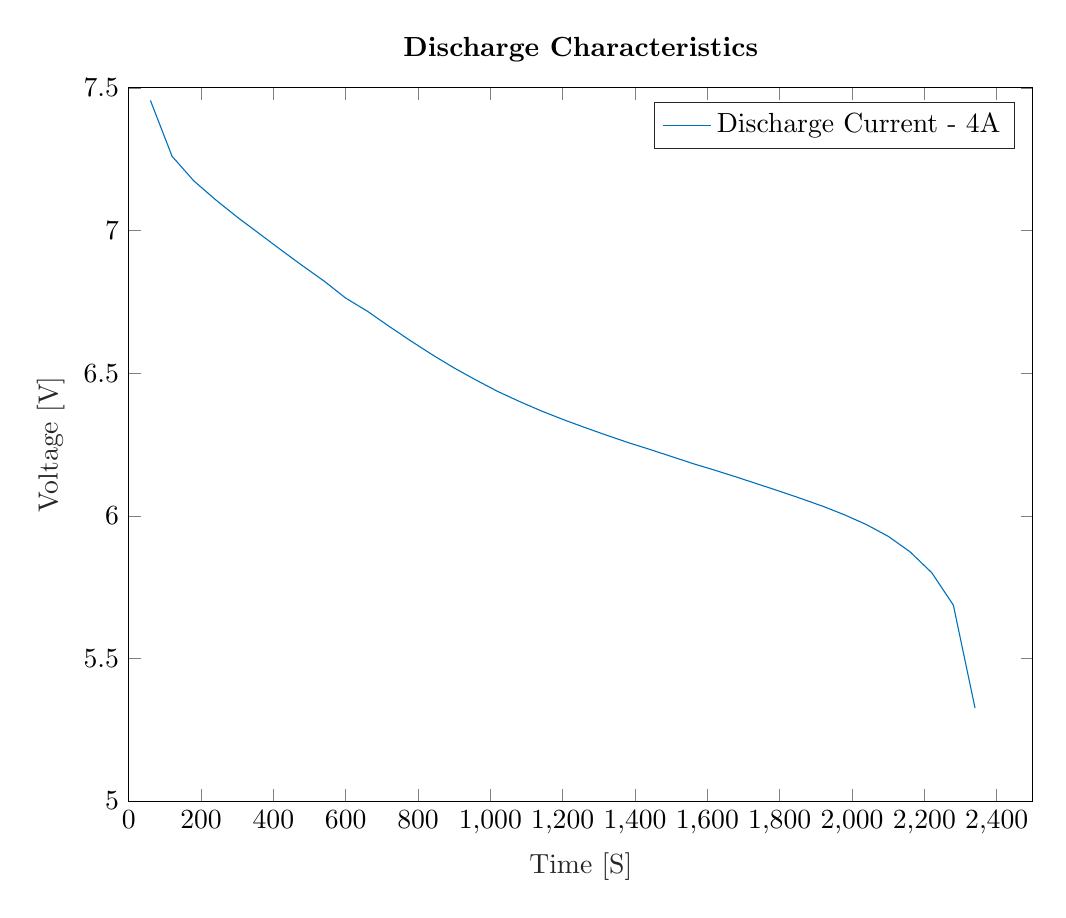
\begin{tikzpicture}

\begin{axis}[%
width=4.521in,
height=3.566in,
at={(0.758in,0.481in)},
scale only axis,
xmin=0,
xmax=2500,
xlabel style={font=\color{white!15!black}},
xlabel={Time [S]},
ymin=5,
ymax=7.5,
ylabel style={font=\color{white!15!black}},
ylabel={Voltage [V]},
axis background/.style={fill=white},
title style={font=\bfseries},
title={Discharge Characteristics},
legend style={legend cell align=left, align=left, draw=white!15!black}
]
\addplot [color=mycolor1]
  table[row sep=crcr]{%
60	7.456\\
120	7.26\\
180	7.174\\
240	7.108\\
300	7.047\\
360	6.99\\
420	6.933\\
480	6.877\\
540	6.823\\
600	6.763\\
660	6.717\\
720	6.664\\
780	6.613\\
840	6.564\\
900	6.518\\
960	6.476\\
1020	6.436\\
1080	6.401\\
1140	6.368\\
1200	6.338\\
1260	6.31\\
1320	6.283\\
1380	6.257\\
1440	6.233\\
1500	6.208\\
1560	6.183\\
1620	6.16\\
1680	6.136\\
1740	6.111\\
1800	6.086\\
1860	6.06\\
1920	6.033\\
1980	6.003\\
2040	5.969\\
2100	5.928\\
2160	5.874\\
2220	5.801\\
2280	5.687\\
2340	5.326\\
};
\addlegendentry{Discharge Current - 4A}

\end{axis}
\end{tikzpicture}%
	\caption{Discharge curve of the Ansmann 18650 2S1P Li-Ion battery used to power the swarmbot.}
	\label{fig:discharge_repeat}
\end{figure}
According to \cite{microzed_hardware_guide} the estimated maximum power draw of the MicroZed is 1.7A at 5V.
This is assuming 85\% utilisation of PL and a conservative 80\% efficiency of the converters.
The estimate made by Avnet is made with the Zynq-7010 in the Xilinx Power Estimator (XPE) \cite{xpe}.
The MicroZed used for the swarmbot project, however, is equipped with the Zynq-7020, a slightly larger chip.
Running the same scenario, 85\% utilisation, in XPE reveals that the 7020 draws 2.3W, just 0.1W more than the 7010, a marginal difference in the total power budget.
In addition to the MicroZed, also the debug LEDs and the microphone board are powered from this rail, adding an estimated $\approx$150mA extra current draw.
In summary, these are the requirements for the DC/DC converter used for generating the 5V rail:

\begin{itemize}
	\item Must function across the entire voltage range of the battery, 6V to 8.4V.
	\item Should be able to supply at least 1.85A at 5V.
\end{itemize}

Below is a discussion of the various choices made in the design of the circuitry of the 5V supply.

\subsubsection*{Designing the 5V Rail}
The PTH08080WAH \cite{pth08080} closely meets these requirements at a maximum power delivery of 2A/10W/5V.
The device is designed to have a wide input range, accepting \texttt{Vin}=\texttt{Vo}+1.1V to 18V.
At the required 5V this translates to an input range of 6.1V to 18V.
This is of course slightly higher than the desired 6V, but even at the maximum discharge rate, estimated at 2.2A-2.3A, with the MicroZed drawing its maximum current and the motors running at full speed, there would still be approximately \thomas{some amount of minutes/hours} minutes of operation per charge.
\texttt{Vo} is determined via an external resistor \texttt{Rset}.
A formulae is provided to calculate the exact \texttt{Rset} needed for a given voltage, however a large table of common values is already calculated.
According to this table, \texttt{Rset}=353$\omega$ results in 5V.
353$\omega$ is not a standard value, choosing 348$\omega$ instead yields 5.01V, which is fine for this application.
\\~\\
The circuit appertaining to this component can be seen in figure \ref{fig:dcdccomponent}.
This is the standard application circuit as shown in the datasheet (figure 10 \cite{pth08080}).
According to the datasheet, the minimum recommended input capacitance is 100$\mu$F. 
Of the capacitors on the list of recommended capacitors, also given in the datasheet, the 20SVP150M was chosen.
It is rated for 20V, sufficient for this application, and has a capacitance of 150$\mu$F. 

\begin{figure}
	\centering
	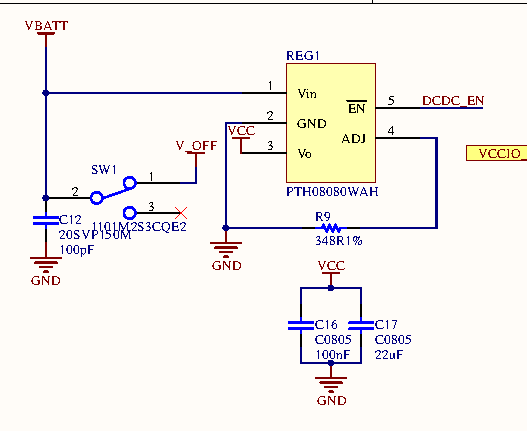
\includegraphics[width=0.7\linewidth]{graphics/5v.pdf}
	\caption{Circuit for generating \texttt{VCC}, the 5V rail.}
	\label{fig:pth08080}
\end{figure}

\subsection{Power Up Sequencing}
On power up the first that needs to happen is to pull the MicroZeds PWR\_EN high on the carrier card.
This is done with a pull-up resistor as shown in figure \ref{fig:pwr_en_circuit}.

\begin{figure}
	\centering
	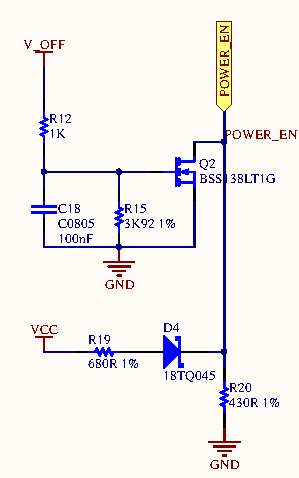
\includegraphics[width=.4\linewidth]{graphics/power_en_sch.pdf}
	\caption{Circuit for proper power sequencing on MicroZeds PWR\_EN.}
	\label{fig:pwr_en_circuit}
\end{figure}

When the MicroZed has powered up its internal DC/DC converters and is ready to receive voltage on its I/O banks the VCCIO\_EN will go high.
VCCIO\_EN has a logic level of 1.8V and the signal is therefore fed to a comparator that outputs a 5V signal to a DC/DC converter when VCCIO\_EN is high.
The DC/DC converter is configured to produce a voltage level of 3.3V that is connected to $V_{ccio}$
This circuitry can be seen in figure \ref{fig:pwr_io_circuit}.

\begin{figure}
	\centering
	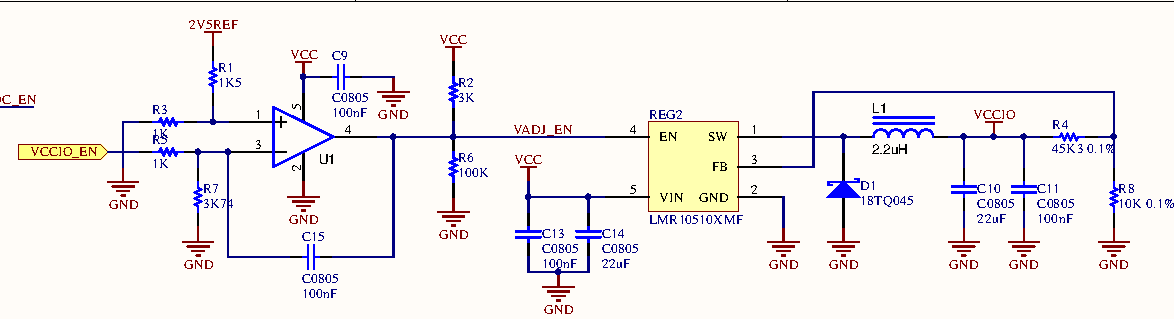
\includegraphics[width=1\linewidth]{graphics/vccio_power_up.pdf}
	\caption{Circuit for proper power sequencing on I/O banks.}
	\label{fig:pwr_io_circuit}
\end{figure}

\subsection{Power Down Sequencing}
\mikkel{Tell why it is important = signal integrity}
On power down VCCIO\_EN, DCDC\_EN and PWR\_EN should be pulled down. 
VCCIO\_EN needs to be pulled down first, hereafter PWR\_EN and lastly DCDC\_EN .
The signals are pulled down by MOSFETS controlled by the V\_OFF signal.
When the power switch on the carrier card is flicked, the battery voltage is connected to the V\_OFF rail thereby turning the MOSFETS on and pulling the signals down. 
The correct sequence is maintained by charging capacitors on the gate side of the MOSFETS thereby creating a delay.
Such a MOSFET circuit is shown in figure \ref{fig:pwr_en_circuit}.

\subsection{Analog to Digital Converter}
The Zynq 7-series FPGA's are equipped with a dual, 12 bit ADC, yet has only one dedicated analog differential pair, \texttt{VP\_0} and \texttt{VN\_0}.
See figure \ref{fig:adc} for an overview of the XADC architechture
If more ADC channels are needed, any of the 16 auxiliary analog inputs (AAI) can be used.
These are placed on I/O bank 35 which, as the rest of the I/O on the swarmbot carrier card, is supplied with \texttt{VCCIO}=3.3V.
Once selected, a multiplexer applies each signal to the ADC's in turn.
For this reason any signal on the AAI can never go above \texttt{VCCIO} to avoid damaging the inputs.
On the swarmbot carrier card the dedicated analog pins, as well as three AAI pairs are routed to the ADC header (\texttt{CON4}).
The signals \texttt{VAUX\_P0} and \texttt{VAUX\_N0} on \texttt{JX1} are the dedicated analog inputs and can be used on its own.
The remaining three pairs are AAI and must be multiplexed if the user wishes to use them.
It should be noted that due to the anti-aliasing filters, these pairs cannot be used as digital I/O on the swarmbot carrier card.
These anti-aliasing filters are required in order to filter out high frequency noise in the differential pairs and should be placed as closely to the Zynq as possible, in this case, that is next to the connectors \texttt{JX1} and \texttt{JX2}, the main connectors to the MicroZed.
Figure \ref{fig:anti_a} from \cite{adch} illustrates a simple measurement setup and the anti-aliasing filter.
\texttt{R1} and \texttt{R2} form a voltage divider, creating a 1V signal.
\texttt{R5} is matched to the parallel impedance of \texttt{R1||R2}.
Resistors \texttt{R3}, \texttt{R4} and the capacitor \texttt{C1} can be adjusted to change the settling time of the circuit.
\cite{adc} gives equation \ref{eq:aliasing} which can be used to calculate the settling time and by that determine the maximum sampling frequency.

\begin{equation}
	\label{eq:aliasing}
	T_{settle}=\log{2^{resolution+1}}\cdot \left(\frac{R1\cdot R2}{R1 + R2}+R3+R4+R5\right)\cdot C_1 = 4.9\cdot 10^{-6}
\end{equation}

\begin{figure}
	\centering
	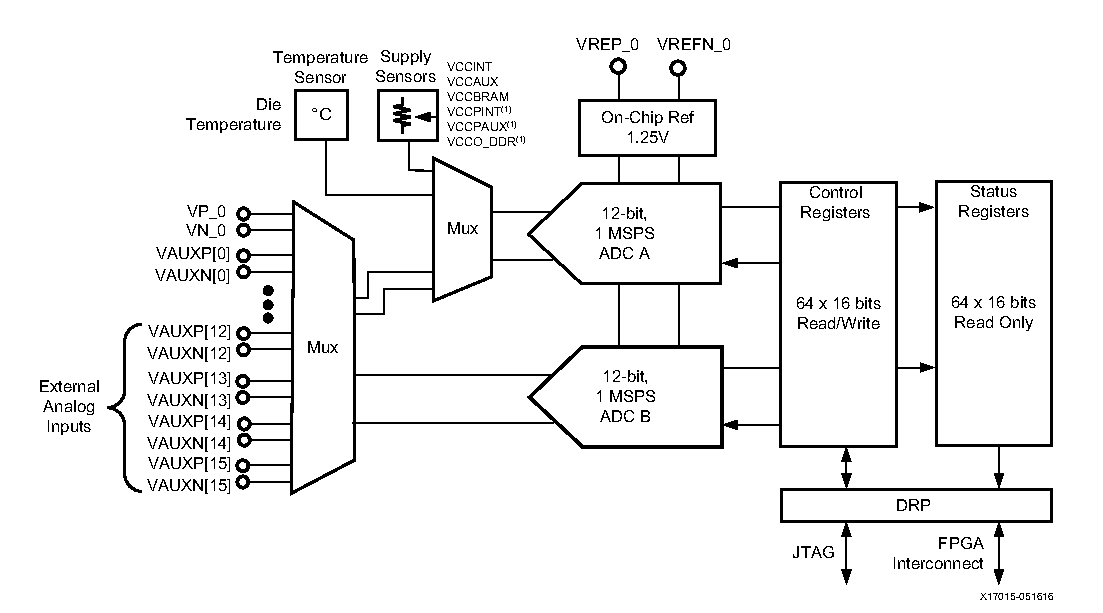
\includegraphics[width=1\linewidth]{graphics/adc.pdf}
	\caption{XADC Block Diagram from Xilinx ADC userguide \cite{adc}.}
	\label{fig:adc}
\end{figure}

\begin{figure}
	\centering
	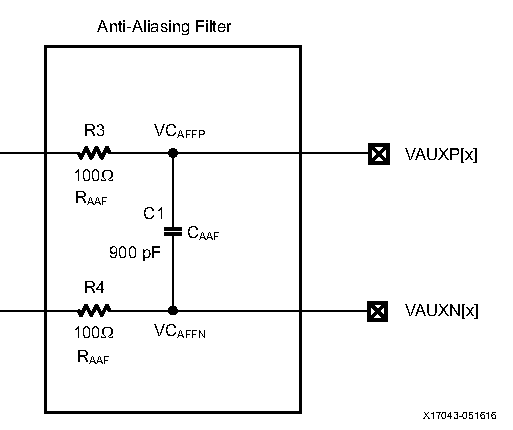
\includegraphics[width=0.8\linewidth]{graphics/anti_aliasing.pdf}
	\caption{Anti-Aliasing diagram from Xilinx ADC userguide \cite{adc}.}
	\label{fig:anti_a}
\end{figure}


\subsection{Buzzer Solution...}	
As described in section \ref{sub:click_generator} it was found that the best solution for creating a click noise on the platform was to use a piezo speaker with a drive circuit and a \texttt{PWM} signal.
But because there has been made no further investigation into what sound level is needed and what the frequency spectrum of the generated click is, it was decided to leave the circuitry out of the carrier card.
Furthermore the sound source should be placed in the center of the robot to ease localization of the robot, but the design of the carrier card did not allow this.
Therefore it was decided to include a header providing access to two IO ports, ground and \texttt{VBATT}.
The header is shown in figure \ref{fig:audio_header}.
Two IO ports are needed if differential drive of the piezo is wanted.
Two holes were added to the carrier card to allow for fixture of the external piezo and drive circuit.

\begin{figure}
	\centering
	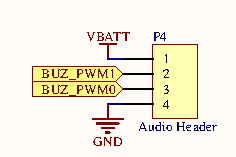
\includegraphics[width=0.4\linewidth]{graphics/audio_header.pdf}
	\caption{Audio header on the carrier card.}
	\label{fig:audio_header}
\end{figure}



\subsection{Pinout}

\subsection{Choice of Components}
As mentioned, the choice of components is largely based upon the Avnet carrier card.
Generally the same components were chosen, but because of pricing, availability or ordering batch size similar components were chosen instead.
Table \ref{tab:components1} and \ref{tab:components2} in appendix \ref{app:components} explains what components were chosen and why.